\documentclass[11pt,a4paper]{jsarticle}
%
\usepackage{amsmath,amssymb}
\usepackage{bm}
\usepackage{graphicx}
\usepackage{ascmac}
\usepackage{listings}
\usepackage{plistings}
\usepackage{url}
%
\setlength{\textwidth}{\fullwidth}
\setlength{\textheight}{40\baselineskip}
\addtolength{\textheight}{\topskip}
\setlength{\voffset}{-0.2in}
\setlength{\topmargin}{0pt}
\setlength{\headheight}{0pt}
\setlength{\headsep}{0pt}
%
\newcommand{\divergence}{\mathrm{div}\,}  %ダイバージェンス
\newcommand{\grad}{\mathrm{grad}\,}  %グラディエント
\newcommand{\rot}{\mathrm{rot}\,}  %ローテーション
%
\title{機械学習関連メモ}
\author{Ryoichi Matsumoto}
\date{\today}
\begin{document}
\maketitle
%
%
\tableofcontents
\listoftables
\listoffigures
%
%

\section{はじめに}
機械学習に関して調べたことのメモ.

\section{Deep Learning}

\subsection{Deep Learningの歴史}

Deep LearningはAIを実現する手段のひとつであり,Deep Learningの歴史の前にAI研究の歴史について概略を説明する.\cite{dl_hist1} \cite{dl_hist2}

AIは図\ref{ai_hist_jpg}に示すように,第一次ブームから第三次ブームがあり,これまでに2回,冬の時代が訪れている.第一次ブームは1950年代~1960年代で,商用コンピュータの登場によりAIの研究が進んだが,人間と同じ考え方を持たせるという理想への壁は高く,1970年代にブームが冷め,1回目の冬の時代が訪れた.第二次ブームは1980年代で,進化したコンピュータに知識を加えるアプローチが行われたが,コンピュータは知識の意味を理解するわけではないため,1990年代にブームが冷め,2回目の冬の時代が訪れた.第三次ブームは2000年代で,インターネットの発展により収集可能なデータの規模が劇的に増加し,AIの研究に活用ができるようになり,機械学習・Deep Learningの研究が加速し,2020年現在もなお,研究が進んでいる.

\begin{figure}
	\begin{center}
		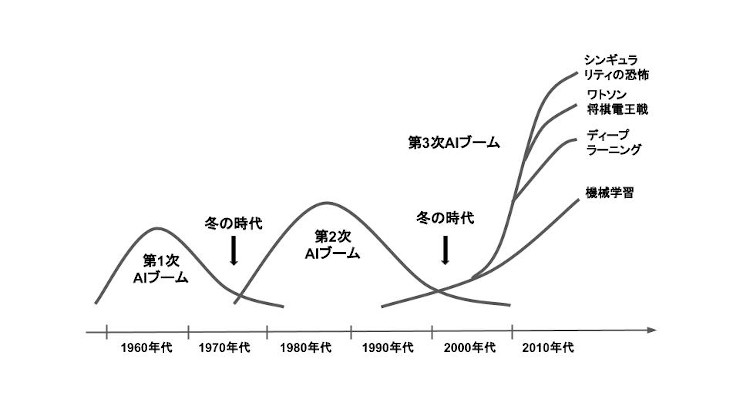
\includegraphics[height=6cm, bb=0 0 160 104]{data/figure/ai_hist.jpg}
		\caption{AIのブームと冬の時代}
		\label{ai_hist_jpg}
	\end{center}
\end{figure}

Deep Learningが最初に脚光を浴びたのは…

\subsection{Batch Normalization}

\subsubsection{背景}
訓練時とテスト時で入力(共変量)の分布が異なる状況は「共変量シフト」と呼ばれ,このような場合は良い学習結果が得られない.共変量シフト下においては,忘却型の学習アルゴリズムやパラメータ学習法,モデル選択法等が用いられる\cite{cov_shift}が,Deep Learningにおいては,学習過程でパラメータ更新により各層のActivationの分布が変わる「内部共変量シフト(Internal Covariate Shift)」と呼ばれる問題がある\cite{bn_abs} \cite{bn_google}.

\subsubsection{概説}
Deep Learningは画像,音声など様々な分野で急速な技術進化をもたらした.Deep Networkの学習方法として確率的勾配降下法(Stochastic gradient descent ; SGD)が効果的であることが知られている\cite{sgd_overview}.SGDの派生として,Momentum,AdaGrad,RMSprop,Adam,AdaBound,RAdamなどがある.SGDはNetworkのパラメータ$\Theta$を,lossを最小化するように最適化する.

\begin{equation}
	\Theta = {\rm arg}\,\underset{\Theta}{\rm min}\frac{1}{N}\sum_{i=1}^{N}l({\rm x}_i, \Theta)
\end{equation}

${\rm x}_{1...N}$はデータ数$N$サンプルの学習データセットで,SGDでの学習ステップは$m$サンプルのミニバッチ${\rm x}_{1...m}$に対して行う.ミニバッチは,パラメータについての損失関数の勾配近似に使用され,式(\ref{approximate_gradient})で導出する.

\begin{equation}
\label{approximate_gradient}
	\frac{1}{m}\frac{\partial l({\rm x}_i, \Theta)}{\partial \Theta}
\end{equation}

SGDでは,学習率をはじめとするハイパーパラメータや,モデルパラメータの初期値の調整が重要である.各層の入力が一つ前の層のモデルパラメータの影響を受け,この影響がネットワークが深いほど大きくなるため,学習が複雑化する.学習によってモデルパラメータが更新され,各層の入力分布が変わり学習の系が変わることで,内部共変量シフトが引き起こされる.この内部共変量シフトを軽減することで学習を安定化する手法の一つがBatch Normalizationである.

ネットワークの一部を切り出して,式(\ref{loss_part_of_network})の損失関数を考える.

\begin{equation}
\label{loss_part_of_network}
	l = F_2(F_1(u, \Theta_1), \Theta_2)
\end{equation}

$F_1,F_2$は任意の変換関数,$\Theta_1,\Theta_2$は損失$l$の最小化により学習されるパラメータである.$\Theta_2$の学習は,入力を${\rm x} = F_1(u, \Theta_1)$とおき,

\begin{equation}
	l = F_2({\rm x}, \Theta_2)
\end{equation}

とすると,パラメータ$\Theta_2$の更新

\begin{equation}
	\Theta_2 \leftarrow \Theta_2 - \frac{\alpha}{m}\sum_{i=1}^{m}\frac{\partial F_2({\rm x}_i, \Theta_2)}{\partial \Theta_2}
\end{equation}

は,入力${\rm x}$の独立したネットワーク$F_2$と等価である.したがって,学習効果を高める入力分布の性質は,学習データとテストデータで同じ分布を持たせることと同様に,サブネットワークの学習に対して有効である.つまり,学習時間経過によらず${\rm x}$の分布を一定に保つことは有効であり,$\Theta_2$の再調整を不要とすることができる.

そこで,各学習ステップでActivationの白色化を行うことを考える.学習後のバイアス$b$を加算し,学習データに対して計算されたActivationの平均で減算した結果で正規化する入力$u$を持つ層は$\hat{x}=x-E[x]$で示される.ここで,$x=u+b,E[x]=\frac{1}{N}\sum_{i=1}^{N}x_i$である.勾配降下ステップが$E[x]$の$b$についての依存がないとき,$b$の更新は$b \leftarrow b+\Delta b$,$\Delta b \propto -\partial l / \partial \hat[x]$で示され,$u+(b+\Delta b)-E[u+(b+\Delta b)]=u+b-E[u+b]$となる.

$d$次元の入力$x=(x^(1) ... x^(d))$を持つネットワークの層について


Batch NormalizationではActivationの出力$x$とペアのパラメータ$\gamma, \beta$を用いて,
\begin{equation}
	y = \gamma x + \beta
\end{equation}

\subsection{You Only Look Once}
You Only Look Once(YOLO)は物体検出手法の一つで,「検出」と「識別」を同時に行うことで,処理時間の遅延を解消することを特長とする.



\section{Section}
...

\subsection{Subsection}
...

\subsection{Subsection}
...


\begin{thebibliography}{9}
	\bibitem{dl_hist1} AI(人工知能)の歴史|時系列で簡単解説, \url{https://ledge.ai/history-of-ai/}
	\bibitem{dl_hist2} 「Deep Learning」の進化でAIを活用した新しいビジネスが生まれる, \url{https://www.nttcom.co.jp/comware_plus/img/201705_DeepLearning.pdf}
	\bibitem{cov_shift} 共変量シフト下での教師付き学習, \url{https://www.jstage.jst.go.jp/article/jnns/13/3/13_3_111/_article/-char/ja/}
	\bibitem{bn_abs} Batch Normalization:ニューラルネットワークの学習を加速させる汎用的で強力な手法, \url{https://deepage.net/deep_learning/2016/10/26/batch_normalization.html}
	\bibitem{bn_google} Batch Normalization: Accelerating Deep Network Training by Reducing Internal Covariate Shift, \url{https://arxiv.org/abs/1502.03167}
	\bibitem{sgd_overview} Optimization: Stochastic Gradient Descent, \url{http://deeplearning.stanford.edu/tutorial/supervised/OptimizationStochasticGradientDescent/}
	\bibitem{yolo_hist} 【物体検出手法の歴史 : YOLOの紹介】, \url{https://qiita.com/mdo4nt6n/items/68dcda71e90321574a2b}
	\bibitem{yolo_hist2} Object Detection YOLO v1 , v2, v3, \url{https://medium.com/@venkatakrishna.jonnalagadda/object-detection-yolo-v1-v2-v3-c3d5eca2312a}
	\bibitem{yolo_v1} You Only Look Once: Unified, Real-Time Object Detection, \url{https://arxiv.org/abs/1506.02640}
	\bibitem{yolo_v2} YOLO9000: Better, Faster, Stronger, \url{https://arxiv.org/abs/1612.08242}
	\bibitem{yolo_v3} YOLOv3: An Incremental Improvement, \url{https://arxiv.org/abs/1804.02767}
\end{thebibliography}

%
%
\end{document}